\section{Proposed Technique}

\subsection{Approach Overview}

\para{Input \& Output.}
We study a long-context coding task in an agentic setting: given (i)~a natural-language issue description and (ii)~access to a software repository at a fixed snapshot, the model interacts with a shell environment over multiple turns, reading files, running tests, and editing code, to produce a patch that resolves the described issue \cite{jimenez2023swebench}. We build on mini-swe-agent \cite{yang2024sweagent}, a minimal agentic framework where the agent repeatedly queries a language model, executes bash commands, and observes the output.

\para{Main Idea.}
Our core idea is to replace the \emph{text} representation of code with an \emph{image} representation wherever the agent encounters source code during its workflow. Concretely, when a tool command returns a code-heavy output (e.g., reading a file via a shell command), we render that output as a monospace document image (see Figure~\ref{fig:rendering-example}) and present it to the vision-capable model as an image input instead of text. This lets us test whether a model can perform multi-step software engineering through the visual channel without any post-training or architectural change.

The key insight is that code reading happens predominantly during the agent loop, not in the initial problem description. Our analysis of agent traces shows that file-reading commands account for over 80\% of the code tokens the model processes, while code blocks in the issue description are a small fraction. Therefore, we apply optical encoding at the \emph{observation level}, intercepting tool outputs, rather than only at the input level.

\subsection{Approach Details}

\para{Observation-Level Optical Encoding.}
At each step of the agent loop, the model issues a bash command, the environment executes it, and the output is returned as a message. In the standard (text) setup, this output is a plain-text string. In our optical setup, we add an intermediate step: if the output is identified as code (see below), we render it as one or more images and present those images to the model in lieu of the text.

A technical constraint shapes the implementation: the OpenAI tool-call API requires tool-response messages to contain only text, not images. We work around this by (1)~replacing the code output in the tool message with a short placeholder (e.g., ``[Code output (243 lines) rendered as image in the next message]'') and (2)~injecting a follow-up user message containing the rendered images. The model thus sees the tool acknowledgment followed immediately by the visual code content.

\para{Code Detection Heuristic.}
Not all tool outputs should be rendered as images; directory listings, error messages, short grep results, and test outputs are better left as text. We apply a simple heuristic: an output is rendered as an image if and only if it satisfies both of the following conditions:
\begin{itemize}[leftmargin=*]
  \item \textbf{Length $>$ 2{,}000 characters}, ensuring that only substantial outputs are converted (short outputs gain little from compression).
  \item \textbf{Code ratio $>$ 20\%}, where ``code ratio'' is the fraction of lines whose stripped content starts with a Python keyword or indentation pattern (def, class, import, from, if, for, return, while, try, \#, or four-space indent).
\end{itemize}

Table~\ref{tab:code-detection-examples} illustrates the heuristic on representative tool outputs from our experiments. In practice, 25\% of all tool outputs are rendered as images (92 out of 366 across 20 pilot instances), and these account for the vast majority of code tokens the model processes.

\begin{table}[t]
\centering
\caption{Examples of the code detection heuristic. Outputs exceeding both thresholds (length $>$ 2{,}000 chars, code ratio $>$ 20\%) are rendered as images; others remain as text.}
\label{tab:code-detection-examples}
\small
\begin{tabular}{p{3.8cm}rrl}
\toprule
\textbf{Command} & \textbf{Chars} & \textbf{Code\%} & \textbf{Action} \\
\midrule
sed -n `1,240p' models.py & 7{,}859 & 31\% & Image \\
cat utils.py & 7{,}574 & 33\% & Image \\
python3 repro.py & 1{,}052 & 35\% & Text \\
grep -n ``def prepare'' & 87 & 0\% & Text \\
ls -la & 1{,}030 & 0\% & Text \\
git diff file.py & 1{,}268 & 6\% & Text \\
\bottomrule
\end{tabular}
\end{table}

\para{Rendering Pipeline.}
Each code output that passes the heuristic is rendered into one or more PNG images using the Python Pillow library. The rendering specification was determined through a systematic pilot study (Section~\ref{sec:rendering-config}): 12pt DejaVu Sans Mono, 120-character page width, 80 lines per image, black text on white background, no syntax highlighting. Files exceeding 80 lines are split across multiple images, each labeled with a header indicating the segment number.

% ------ Algorithm 1: Optical Encoding Pipeline ------
\begin{algorithm}[t]
\caption{Observation-Level Optical Encoding}\label{alg:optical}
\KwInput{Tool output text $t$, rendering parameters $\theta$}
\KwOutput{Message sequence $\mathcal{M}$ (tool message + optional image message)}
$r \leftarrow \mathrm{code\_ratio}(t)$\;
\uIf{$|t| > 2000$ \textbf{and} $r > 0.2$}{
  $n \leftarrow |\mathrm{lines}(t)|$\;
  $\mathit{chunks} \leftarrow \textsc{SplitByLines}(t,\; \theta.\mathit{max\_lines})$\;
  $\mathit{images} \leftarrow [\textsc{Render}(c, \theta) \text{ for } c \in \mathit{chunks}]$\;
  $m_{\mathrm{tool}} \leftarrow \text{``[Code output (}n\text{ lines) rendered as image]''}$\;
  $m_{\mathrm{img}} \leftarrow \textsc{UserMessage}(\mathit{images})$\;
  \Return{$(m_{\mathrm{tool}},\; m_{\mathrm{img}})$}
}{
  \Return{$(\textsc{ToolMessage}(t),)$} \tcp*{keep as text}
}
\end{algorithm}

Algorithm~\ref{alg:optical} summarizes the decision logic applied at each agent step. For outputs classified as code, the tool message contains a placeholder and a follow-up user message delivers the rendered images. For all other outputs, the original text is passed through unchanged.

\begin{figure}[t]
  \centering
  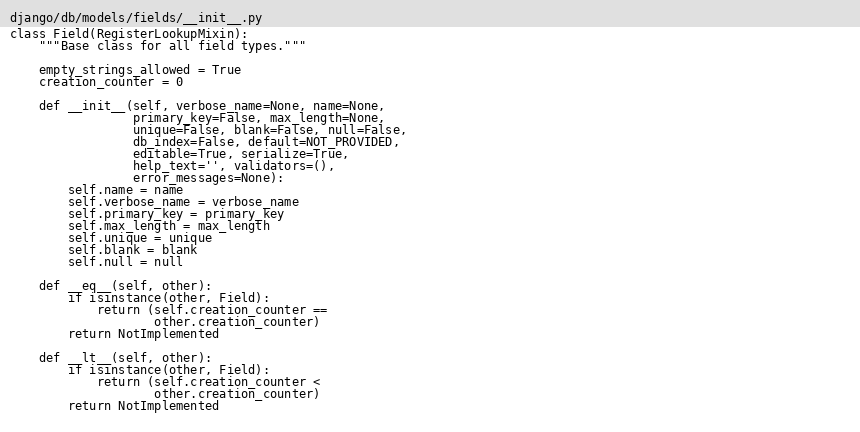
\includegraphics[width=\linewidth]{Sections/figures/rendering_example.png}
  \caption{Example of a rendered code image as seen by the model. The agent issued a file-read command; the output was detected as code (31\% code ratio, 7{,}859 characters) and rendered at 12pt/120-char width.}
  \label{fig:rendering-example}
\end{figure}

\para{Integration with mini-swe-agent.}
We implement the optical encoding as a subclass of the default agent (OpticalAgent) that overrides the action-execution method. The agent loop proceeds as follows: (1)~the model receives the conversation history and generates a bash command via tool call; (2)~the environment executes the command and returns the output; (3)~the OpticalAgent checks whether the output passes the code detection heuristic; (4a)~if yes, the output is rendered as images, the tool message is replaced with a placeholder, and a user message with the images is appended; (4b)~if no, the output is passed as text normally; (5)~the model sees the updated history and generates the next command. This cycle repeats until the model submits a patch or hits the step/cost limit.

This design requires no changes to the framework's core code, model interface, or environment layer. The same prompt template, decoding settings, and evaluation protocol are used for both conditions, ensuring that the input representation is the only experimental variable. The issue description (problem statement) is also preprocessed: markdown code blocks are rendered as images using the same pipeline.
